% Options for packages loaded elsewhere
\PassOptionsToPackage{unicode}{hyperref}
\PassOptionsToPackage{hyphens}{url}
\PassOptionsToPackage{dvipsnames,svgnames*,x11names*}{xcolor}
%
\documentclass[
  11pt,
  ignorenonframetext,
  aspectratio=169,
  aspectratio=169]{beamer}
\usepackage{pgfpages}
\setbeamertemplate{caption}[numbered]
\setbeamertemplate{caption label separator}{: }
\setbeamercolor{caption name}{fg=normal text.fg}
\beamertemplatenavigationsymbolsempty

%%
%%% Definition of colors
%%% Source: https://latexcolor.com/
\definecolor{blanchedalmond}{rgb}{1.0, 0.92, 0.8}
\definecolor{blond}{rgb}{0.98, 0.94, 0.75}
%%% End of definition of colors
%%

% Prevent slide breaks in the middle of a paragraph
\widowpenalties 1 10000
\raggedbottom
\usepackage{lmodern}
\usepackage{amssymb,amsmath}
\usepackage{ifxetex,ifluatex}
\ifnum 0\ifxetex 1\fi\ifluatex 1\fi=0 % if pdftex
  \usepackage[T1]{fontenc}
  \usepackage[utf8]{inputenc}
  \usepackage{textcomp} % provide euro and other symbols
\else % if luatex or xetex
  \usepackage{unicode-math}
  \defaultfontfeatures{Scale=MatchLowercase}
  \defaultfontfeatures[\rmfamily]{Ligatures=TeX,Scale=1}
  \setmainfont[]{STSong}
  \ifxetex
    \usepackage{xeCJK}
    \setCJKmainfont[]{STSong}
  \fi
  \ifluatex
    \usepackage[]{luatexja-fontspec}
    \setmainjfont[]{STSong}
  \fi
\fi
\usetheme[]{Frankfurt}
\usecolortheme{beaver}
\usefonttheme{professionalfonts}
\usefonttheme{serif} % use mainfont rather than sansfont for slide text
% Use upquote if available, for straight quotes in verbatim environments
\IfFileExists{upquote.sty}{\usepackage{upquote}}{}
\IfFileExists{microtype.sty}{% use microtype if available
  \usepackage[]{microtype}
  \UseMicrotypeSet[protrusion]{basicmath} % disable protrusion for tt fonts
}{}
\makeatletter
\@ifundefined{KOMAClassName}{% if non-KOMA class
  \IfFileExists{parskip.sty}{%
    \usepackage{parskip}
  }{% else
    \setlength{\parindent}{0pt}
    \setlength{\parskip}{6pt plus 2pt minus 1pt}}
}{% if KOMA class
  \KOMAoptions{parskip=half}}
\makeatother
\usepackage{xcolor}
\IfFileExists{xurl.sty}{\usepackage{xurl}}{} % add URL line breaks if available
\IfFileExists{bookmark.sty}{\usepackage{bookmark}}{\usepackage{hyperref}}
\hypersetup{
  pdftitle={My wonderful presentation},
  pdfauthor={Alexey Gumirov},
  colorlinks=true,
  linkcolor=Maroon,
  filecolor=Maroon,
  citecolor=Blue,
  urlcolor=red,
  pdfcreator={LaTeX via pandoc}}
\urlstyle{same} % disable monospaced font for URLs
\newif\ifbibliography
\usepackage{listings}
\newcommand{\passthrough}[1]{#1}
\lstset{defaultdialect=sh}
\lstset{framexleftmargin=0mm, frame=trBL,backgroundcolor=\color{blanchedalmond!5},numbers=left,numberstyle=\scriptsize,basicstyle=\small}
\lstset{aboveskip=5mm,belowskip=5mm,xleftmargin=20pt,xrightmargin=5pt}
% \lstset{prebreak={\raisebox{0ex}[0ex][0ex]}}
% \lstset{postbreak={\raisebox{0ex}[0ex][0ex]\space}}
\lstset{breaklines=true,breakatwhitespace=true}
\usepackage{longtable,booktabs}
\usepackage{caption}
% Make caption package work with longtable
\makeatletter
\def\fnum@table{\tablename~\thetable}
\makeatother
\usepackage{graphicx,grffile}
\makeatletter
\def\maxwidth{\ifdim\Gin@nat@width>\linewidth\linewidth\else\Gin@nat@width\fi}
\def\maxheight{\ifdim\Gin@nat@height>\textheight\textheight\else\Gin@nat@height\fi}
\makeatother
% Scale images if necessary, so that they will not overflow the page
% margins by default, and it is still possible to overwrite the defaults
% using explicit options in \includegraphics[width, height, ...]{}
\setkeys{Gin}{width=\maxwidth,height=\maxheight,keepaspectratio}
% Set default figure placement to htbp
\makeatletter
\def\fps@figure{htbp}
\makeatother
\setlength{\emergencystretch}{3em} % prevent overfull lines
\providecommand{\tightlist}{%
  \setlength{\itemsep}{0pt}\setlength{\parskip}{0pt}}
\setcounter{secnumdepth}{-\maxdimen} % remove section numbering

%
% When using babel or polyglossia with biblatex, loading csquotes is recommended 
% to ensure that quoted texts are typeset according to the rules of your main language.
%
\usepackage{csquotes}

%
% blockquote
%
\definecolor{blockquote-border}{RGB}{221,221,221}
\definecolor{blockquote-text}{RGB}{89,89,89}
\usepackage{mdframed}
\newmdenv[rightline=false,bottomline=false,topline=false,linewidth=3pt,linecolor=blockquote-border,skipabove=\parskip]{customblockquote}
\renewenvironment{quote}{\begin{customblockquote}\list{}{\rightmargin=0em\leftmargin=0em}%
\item\relax\color{blockquote-text}\ignorespaces}{\unskip\unskip\endlist\end{customblockquote}}

%
% Source Sans Pro as the de­fault font fam­ily
% Source Code Pro for monospace text
%
% 'default' option sets the default 
% font family to Source Sans Pro, not \sfdefault.
%


\usepackage[normalem]{ulem}
\newcommand{\st}[1]{\sout{#1}}
\pdfstringdefDisableCommands{\renewcommand{\sout}{}}

%%%%%%%%%%%%%color 
\definecolor{UBCblue}{rgb}{0.04706, 0.13725, 0.26667} % UBC Blue (primary)
\definecolor{UBCgrey}{rgb}{0.3686, 0.5255, 0.6235} % UBC Grey (secondary)

\definecolor{orange}{RGB}{244,167,66}

\setbeamercolor{palette primary}{bg=UBCblue,fg=white}
\setbeamercolor{palette secondary}{bg=UBCblue,fg=white}
\setbeamercolor{palette tertiary}{bg=UBCblue,fg=white}
\setbeamercolor{palette quaternary}{bg=UBCblue,fg=white}
\setbeamercolor{structure}{fg=UBCblue} % itemize, enumerate, etc
\setbeamercolor{section in toc}{fg=UBCblue} % TOC sections

%% change circle miniframes color
\setbeamercolor{mini frame}{fg=orange, bg=UBCblue}

%% Change subsection in footer color (author and institute color)
\setbeamercolor{subsection in head/foot}{bg=UBCgrey,fg=white}

%change ilmenau section dot color 
\setbeamercolor{section in head/foot}{fg=orange} 

%% Change the circle in miniframes to a box
%\setbeamertemplate{mini frame}[box]
%\setbeamertemplate{mini frame in current subsection}[box]

%%%%%%%%%%%%%%%%%%%%%%%%%%%%%%%%%%%%%%
%%%% Create framenumber in footer
\newcommand{\frameofframes}{/}
\newcommand{\setframeofframes}[1]{\renewcommand{\frameofframes}{#1}}

\setframeofframes{of}
\makeatletter
\setbeamertemplate{footline}
  {%
    \begin{beamercolorbox}[colsep=1.5pt]{upper separation line foot}
    \end{beamercolorbox}
    \begin{beamercolorbox}[ht=2.5ex,dp=1.125ex,%
      leftskip=.3cm,rightskip=.3cm plus1fil]{author in head/foot}%
      \leavevmode{\usebeamerfont{author in head/foot}\insertshortauthor}%
      \hfill%
      {\usebeamerfont{institute in head/foot}\usebeamercolor[fg]{institute in head/foot}\insertshortinstitute}%
    \end{beamercolorbox}%
    \begin{beamercolorbox}[ht=2.5ex,dp=1.125ex,%
      leftskip=.3cm,rightskip=.3cm plus1fil]{title in head/foot}%
      {\usebeamerfont{title in head/foot}\insertshorttitle}%
      \hfill%
      {\usebeamerfont{frame number}\usebeamercolor[fg]{frame number}\insertframenumber~\frameofframes~\inserttotalframenumber}
    \end{beamercolorbox}%
    \begin{beamercolorbox}[colsep=1.5pt]{lower separation line foot}
    \end{beamercolorbox}
  }
%%%%%%%%%%%%%%%%%%%%%%%%%%%%%%%%%
%%% Remove subsection bar in mini frames
\defbeamertemplate*{headline}{miniframes theme no subsection}
{%
  \begin{beamercolorbox}[colsep=1.5pt]{upper separation line head}
  \end{beamercolorbox}
  \begin{beamercolorbox}{section in head/foot}
    \vskip2pt\insertnavigation{\paperwidth}\vskip2pt
  \end{beamercolorbox}%
  \begin{beamercolorbox}[colsep=1.5pt]{lower separation line head}
  \end{beamercolorbox}
}

\setbeamertemplate{footline}[miniframes theme no subsection]
%%%%%%%%%%%%%%%%%%%%%%%%%%%
\makeatother

\title{My wonderful presentation}
\author{Alexey Gumirov}
\date{06 一月 2025}
\institute{My home office}
\titlegraphic{
\includegraphics{img/aleph0.png}}
\logo{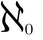
\includegraphics{img/aleph0-small.png}}

\begin{document}
\frame{\titlepage}

\begin{frame}
  \tableofcontents[hideallsubsections]
\end{frame}
\section{General information beamer}\label{general-information-beamer}

\begin{frame}{Themes, fonts, etc. beamer}
\phantomsection\label{themes-fonts-etc.-beamer}
\begin{itemize}
\tightlist
\item
  I use default \textbf{pandoc} themes.
\item
  This presentation is made with \textbf{Frankfurt} theme and
  \textbf{beaver} color theme.
\item
  I like \textbf{professionalfonts} font scheme.
\end{itemize}
\end{frame}

\begin{frame}{Links beamer}
\phantomsection\label{links-beamer}
\begin{itemize}
\tightlist
\item
  Matrix of beamer themes:
  \url{https://hartwork.org/beamer-theme-matrix/}
\item
  Font themes:
  \href{http://www.deic.uab.es/~iblanes/beamer_gallery/index_by_font.html}{http://www.deic.uab.es/\textasciitilde iblanes/beamer\emph{gallery/index}by\_font.html}
\item
  Nerd Fonts: \url{https://nerdfonts.com}
\end{itemize}
\end{frame}

\section{Formatting beamer}\label{formatting-beamer}

\begin{frame}{Text formatting beamer}
\phantomsection\label{text-formatting-beamer}
Normal text. \emph{Italic text} and \textbf{bold text}. \st{Strike} is
supported.
\end{frame}

\begin{frame}{Notes beamer}
\phantomsection\label{notes-beamer}
\begin{quote}
This is a note.

\begin{quote}
Nested notes are not supported. And it continues.
\end{quote}
\end{quote}
\end{frame}

\begin{frame}{Blocks}
\phantomsection\label{blocks}
\begin{itemize}
\tightlist
\item
  Line A
\item
  Line B
\end{itemize}

New block without header.

\begin{block}{This is a block B. beamer}
\phantomsection\label{this-is-a-block-b.-beamer}
\begin{itemize}
\tightlist
\item
  Line C
\item
  Line D
\end{itemize}
\end{block}
\end{frame}

\begin{frame}[fragile]{Listings}
\phantomsection\label{listings}
Listings out of the block.

\begin{lstlisting}[language=sh]
#!/bin/bash
echo "Hello world!"
echo "line"
\end{lstlisting}

\begin{block}{Listings in the block. beamer}
\phantomsection\label{listings-in-the-block.-beamer}
\begin{lstlisting}[language=sh]
#!/bin/bash
echo "Hello world!"
echo "line"
\end{lstlisting}
\end{block}
\end{frame}

\begin{frame}{Table}
\phantomsection\label{table}
\begin{longtable}[]{@{}lrc@{}}
\toprule\noalign{}
\textbf{Item} & \textbf{Description} & \textbf{Q-ty} \\
\midrule\noalign{}
\endhead
Item A & Item A description & 2 \\
Item B & Item B description & 5 \\
Item C & N/A & 100 \\
\bottomrule\noalign{}
\end{longtable}
\end{frame}

\begin{frame}[fragile]{Single picture}
\phantomsection\label{single-picture}
This is how we insert picture. Caption is produced automatically from
the alt text.

\begin{lstlisting}
![Aleph 0](img/aleph0.png) 
\end{lstlisting}

\begin{figure}
\centering

\includegraphics{img/aleph0.png}
\caption{Aleph 0}
\end{figure}
\end{frame}

\begin{frame}[fragile]{Two or more pictures in a raw}
\phantomsection\label{two-or-more-pictures-in-a-raw}
Here are two pictures in the raw. We can also change two pictures size
(height or width).

\begin{lstlisting}
![](img/aleph0.png){height=10%}\ ![](img/aleph0.png){height=30%} 
\end{lstlisting}


\includegraphics[width=\textwidth,height=0.1\textheight]{img/aleph0.png}~
\includegraphics[width=\textwidth,height=0.3\textheight]{img/aleph0.png}
\end{frame}

\begin{frame}{Lists}
\phantomsection\label{lists}
\begin{enumerate}
\tightlist
\item
  Idea 1
\item
  Idea 2

  \begin{itemize}
  \tightlist
  \item
    genius idea A
  \item
    more genius 2
  \end{itemize}
\item
  Conclusion
\end{enumerate}
\end{frame}

\begin{frame}{Two columns of equal width}
\phantomsection\label{two-columns-of-equal-width}
\begin{columns}[T]
\begin{column}{0.48\textwidth}
Left column text.

Another text line.
\end{column}

\begin{column}{0.48\textwidth}
\begin{itemize}
\tightlist
\item
  Item 1.
\item
  Item 2.
\item
  Item 3.
\end{itemize}
\end{column}
\end{columns}
\end{frame}

\begin{frame}{Two columns of with 40:60 split}
\phantomsection\label{two-columns-of-with-4060-split}
\begin{columns}[T]
\begin{column}{0.4\textwidth}
Left column text.

Another text line.
\end{column}

\begin{column}{0.6\textwidth}
\begin{itemize}
\tightlist
\item
  Item 1.
\item
  Item 2.
\item
  Item 3.
\end{itemize}
\end{column}
\end{columns}
\end{frame}

\begin{frame}{Three columns with equal split}
\phantomsection\label{three-columns-with-equal-split}
\begin{columns}[T]
\begin{column}{0.48\textwidth}
Left column text.

Another text line.
\end{column}

\begin{column}{0.48\textwidth}
Middle column list:

\begin{enumerate}
\tightlist
\item
  Item 1.
\item
  Item 2.
\end{enumerate}
\end{column}

\begin{column}{0.48\textwidth}
Right column list:

\begin{itemize}
\tightlist
\item
  Item 1.
\item
  Item 2.
\end{itemize}
\end{column}
\end{columns}
\end{frame}

\begin{frame}{Three columns with 30:40:30 split}
\phantomsection\label{three-columns-with-304030-split}
\begin{columns}[T]
\begin{column}{0.3\textwidth}
Left column text.

Another text line.
\end{column}

\begin{column}{0.4\textwidth}
Middle column list:

\begin{enumerate}
\tightlist
\item
  Item 1.
\item
  Item 2.
\end{enumerate}
\end{column}

\begin{column}{0.3\textwidth}
Right column list:

\begin{itemize}
\tightlist
\item
  Item 1.
\item
  Item 2.
\end{itemize}
\end{column}
\end{columns}
\end{frame}

\begin{frame}{Two columns: image and text}
\phantomsection\label{two-columns-image-and-text}
\begin{columns}[T]
\begin{column}{0.48\textwidth}

\includegraphics[width=\textwidth,height=0.5\textheight]{img/aleph0.png}
\end{column}

\begin{column}{0.48\textwidth}
Text in the right column.

List from the right column:

\begin{itemize}
\tightlist
\item
  Item 1.
\item
  Item 2.
\end{itemize}
\end{column}
\end{columns}
\end{frame}

\begin{frame}{Two columns: image and table}
\phantomsection\label{two-columns-image-and-table}
\begin{columns}[T]
\begin{column}{0.48\textwidth}

\includegraphics[width=\textwidth,height=0.5\textheight]{img/aleph0.png}
\end{column}

\begin{column}{0.48\textwidth}
\begin{longtable}[]{@{}lc@{}}
\toprule\noalign{}
\textbf{Item} & \textbf{Option} \\
\midrule\noalign{}
\endhead
Item 1 & Option 1 \\
Item 2 & Option 2 \\
\bottomrule\noalign{}
\end{longtable}
\end{column}
\end{columns}
\end{frame}

\begin{frame}{Fancy layout}
\phantomsection\label{fancy-layout}
\begin{itemize}
\tightlist
\item
  Point A
\item
  Point B
\end{itemize}

\begin{columns}[T]
\begin{column}{0.48\textwidth}
\begin{itemize}
\tightlist
\item
  Good
\item
  Better
\item
  Best
\end{itemize}
\end{column}

\begin{column}{0.48\textwidth}
\begin{block}{Cons beamer}
\phantomsection\label{cons-beamer}
\begin{itemize}
\tightlist
\item
  Bad
\item
  Worse
\item
  Worst
\end{itemize}
\end{block}
\end{column}
\end{columns}

\begin{block}{Conclusion beamer}
\phantomsection\label{conclusion-beamer}
\begin{itemize}
\tightlist
\item
  Let's go for it!
\item
  No way we go for it!
\end{itemize}
\end{block}
\end{frame}

\end{document}
% Options for packages loaded elsewhere
\PassOptionsToPackage{unicode}{hyperref}
\PassOptionsToPackage{hyphens}{url}
\PassOptionsToPackage{dvipsnames,svgnames,x11names}{xcolor}
\documentclass[
  11pt,
  ignorenonframetext,
  aspectratio=169]{beamer}
\newif\ifbibliography
\usepackage{pgfpages}
\setbeamertemplate{caption}[numbered]
\setbeamertemplate{caption label separator}{: }
\setbeamercolor{caption name}{fg=normal text.fg}
\beamertemplatenavigationsymbolsempty
% remove section numbering
\setbeamertemplate{part page}{
  \centering
  \begin{beamercolorbox}[sep=16pt,center]{part title}
    \usebeamerfont{part title}\insertpart\par
  \end{beamercolorbox}
}
\setbeamertemplate{section page}{
  \centering
  \begin{beamercolorbox}[sep=12pt,center]{section title}
    \usebeamerfont{section title}\insertsection\par
  \end{beamercolorbox}
}
\setbeamertemplate{subsection page}{
  \centering
  \begin{beamercolorbox}[sep=8pt,center]{subsection title}
    \usebeamerfont{subsection title}\insertsubsection\par
  \end{beamercolorbox}
}
% Prevent slide breaks in the middle of a paragraph
\widowpenalties 1 10000
\raggedbottom
\AtBeginPart{
  \frame{\partpage}
}
\AtBeginSection{
  \ifbibliography
  \else
    \frame{\sectionpage}
  \fi
}
\AtBeginSubsection{
  \frame{\subsectionpage}
}
\usepackage{iftex}
\ifPDFTeX
  \usepackage[T1]{fontenc}
  \usepackage[utf8]{inputenc}
  \usepackage{textcomp} % provide euro and other symbols
\else % if luatex or xetex
  \usepackage{unicode-math} % this also loads fontspec
  \defaultfontfeatures{Scale=MatchLowercase}
  \defaultfontfeatures[\rmfamily]{Ligatures=TeX,Scale=1}
\fi
\usepackage{lmodern}
\ifPDFTeX\else
  % xetex/luatex font selection
\fi
% Use upquote if available, for straight quotes in verbatim environments
\IfFileExists{upquote.sty}{\usepackage{upquote}}{}
\IfFileExists{microtype.sty}{% use microtype if available
  \usepackage[]{microtype}
  \UseMicrotypeSet[protrusion]{basicmath} % disable protrusion for tt fonts
}{}
\makeatletter
\@ifundefined{KOMAClassName}{% if non-KOMA class
  \IfFileExists{parskip.sty}{%
    \usepackage{parskip}
  }{% else
    \setlength{\parindent}{0pt}
    \setlength{\parskip}{6pt plus 2pt minus 1pt}}
}{% if KOMA class
  \KOMAoptions{parskip=half}}
\makeatother
\usepackage{listings}
\newcommand{\passthrough}[1]{#1}
\lstset{defaultdialect=[5.3]Lua}
\lstset{defaultdialect=[x86masm]Assembler}
\usepackage{longtable,booktabs,array}
\usepackage{calc} % for calculating minipage widths
\usepackage{caption}
% Make caption package work with longtable
\makeatletter
\def\fnum@table{\tablename~\thetable}
\makeatother
\usepackage{graphicx}
\makeatletter
\newsavebox\pandoc@box
\newcommand*\pandocbounded[1]{% scales image to fit in text height/width
  \sbox\pandoc@box{#1}%
  \Gscale@div\@tempa{\textheight}{\dimexpr\ht\pandoc@box+\dp\pandoc@box\relax}%
  \Gscale@div\@tempb{\linewidth}{\wd\pandoc@box}%
  \ifdim\@tempb\p@<\@tempa\p@\let\@tempa\@tempb\fi% select the smaller of both
  \ifdim\@tempa\p@<\p@\scalebox{\@tempa}{\usebox\pandoc@box}%
  \else\usebox{\pandoc@box}%
  \fi%
}
% Set default figure placement to htbp
\def\fps@figure{htbp}
\makeatother
\setlength{\emergencystretch}{3em} % prevent overfull lines
\providecommand{\tightlist}{%
  \setlength{\itemsep}{0pt}\setlength{\parskip}{0pt}}
\usepackage{bookmark}
\IfFileExists{xurl.sty}{\usepackage{xurl}}{} % add URL line breaks if available
\urlstyle{same}
\hypersetup{
  pdftitle={一次输入,多重输出},
  pdfauthor={CHEN,Xiaoqiang(陈孝强)},
  colorlinks=true,
  linkcolor={Maroon},
  filecolor={Maroon},
  citecolor={Blue},
  urlcolor={red},
  pdfcreator={LaTeX via pandoc}}

\title{一次输入,多重输出}
\author{CHEN,Xiaoqiang(陈孝强)}
\date{2024-01-01}
\institute{粑粑柑共同体}

\begin{document}
\frame{\titlepage}

\begin{frame}[allowframebreaks]
  \setcounter{tocdepth}{3}
  \tableofcontents
\end{frame}
\setcounter{tocdepth}{3}
\tableofcontents
}
\section{介绍}\label{ux4ecbux7ecd}

\begin{frame}{Themes, fonts, etc.}
\phantomsection\label{themes-fonts-etc.}
\begin{itemize}
\tightlist
\item
  I use default \textbf{pandoc} themes.
\item
  This presentation is made with \textbf{Frankfurt} theme and
  \textbf{beaver} color theme.
\item
  I like \textbf{professionalfonts} font scheme.
\end{itemize}
\end{frame}

\begin{frame}{Links}
\phantomsection\label{links}
\begin{itemize}
\tightlist
\item
  Matrix of beamer themes:
  \url{https://hartwork.org/beamer-theme-matrix/}
\item
  Font themes:
  \url{http://www.deic.uab.es/~iblanes/beamer_gallery/index_by_font.html}
\item
  Nerd Fonts: \url{https://nerdfonts.com}
\end{itemize}
\end{frame}

\section{Formatting beamer}\label{formatting-beamer}

\begin{frame}{Text formatting}
\phantomsection\label{text-formatting}
Normal text. \emph{Italic text} and \textbf{bold text}.
\end{frame}

\begin{frame}{Notes}
\phantomsection\label{notes}
\begin{quote}
This is a note.

\begin{quote}
Nested notes are not supported. And it continues.
\end{quote}
\end{quote}
\end{frame}

\begin{frame}{Blocks}
\phantomsection\label{blocks}
\begin{block}{This is a block A}
\phantomsection\label{this-is-a-block-a}
\begin{itemize}
\tightlist
\item
  Line A
\item
  Line B
\end{itemize}

New block without header.
\end{block}

\begin{block}{This is a block B.}
\phantomsection\label{this-is-a-block-b.}
\begin{itemize}
\tightlist
\item
  Line C
\item
  Line D
\end{itemize}
\end{block}
\end{frame}

\begin{frame}[fragile]{Listings}
\phantomsection\label{listings}
Listings out of the block.

\begin{lstlisting}[language=sh]
#!/bin/bash
echo "Hello world!"
echo "line"
\end{lstlisting}

\begin{block}{Listings in the block.}
\phantomsection\label{listings-in-the-block.}
\begin{lstlisting}[language=sh]
#!/bin/bash
echo "Hello world!"
echo "line"
\end{lstlisting}
\end{block}
\end{frame}

\begin{frame}{Table}
\phantomsection\label{table}
\begin{longtable}[]{@{}lrc@{}}
\toprule\noalign{}
\textbf{Item} & \textbf{Description} & \textbf{Q-ty} \\
\midrule\noalign{}
\endhead
Item A & Item A description & 2 \\
Item B & Item B description & 5 \\
Item C & N/A & 100 \\
\bottomrule\noalign{}
\end{longtable}
\end{frame}

\begin{frame}[fragile]{Single picture}
\phantomsection\label{single-picture}
This is how we insert picture. Caption is produced automatically from
the alt text.

\begin{lstlisting}
![Aleph 0](img/aleph0.png) 
\end{lstlisting}

\begin{figure}
\centering
\pandocbounded{
\includegraphics[keepaspectratio]{img/aleph0.png}}
\caption{Aleph 0}
\end{figure}
\end{frame}

\begin{frame}[fragile]{Two or more pictures in a raw}
\phantomsection\label{two-or-more-pictures-in-a-raw}
Here are two pictures in the raw. We can also change two pictures size
(height or width).

\begin{lstlisting}
![](img/aleph0.png){height=10%}\ ![](img/aleph0.png){height=30%} 
\end{lstlisting}


\includegraphics[width=\linewidth,height=0.1\textheight,keepaspectratio]{img/aleph0.png}~
\includegraphics[width=\linewidth,height=0.3\textheight,keepaspectratio]{img/aleph0.png}
\end{frame}

\begin{frame}{Lists}
\phantomsection\label{lists}
\begin{enumerate}
\tightlist
\item
  Idea 1
\item
  Idea 2

  \begin{itemize}
  \tightlist
  \item
    genius idea A
  \item
    more genius 2
  \end{itemize}
\item
  Conclusion
\end{enumerate}
\end{frame}

\begin{frame}{Two columns of equal width}
\phantomsection\label{two-columns-of-equal-width}
\begin{columns}[T]
\begin{column}{0.48\linewidth}
Left column text.

Another text line.
\end{column}

\begin{column}{0.48\linewidth}
\begin{itemize}
\tightlist
\item
  Item 1.
\item
  Item 2.
\item
  Item 3.
\end{itemize}
\end{column}
\end{columns}
\end{frame}

\begin{frame}{Two columns of with 40:60 split}
\phantomsection\label{two-columns-of-with-4060-split}
\begin{columns}[T]
\begin{column}{0.4\linewidth}
Left column text.

Another text line.
\end{column}

\begin{column}{0.6\linewidth}
\begin{itemize}
\tightlist
\item
  Item 1.
\item
  Item 2.
\item
  Item 3.
\end{itemize}
\end{column}
\end{columns}
\end{frame}

\begin{frame}{Three columns with equal split}
\phantomsection\label{three-columns-with-equal-split}
\begin{columns}[T]
\begin{column}{0.48\linewidth}
Left column text.

Another text line.
\end{column}

\begin{column}{0.48\linewidth}
Middle column list:

\begin{enumerate}
\tightlist
\item
  Item 1.
\item
  Item 2.
\end{enumerate}
\end{column}

\begin{column}{0.48\linewidth}
Right column list:

\begin{itemize}
\tightlist
\item
  Item 1.
\item
  Item 2.
\end{itemize}
\end{column}
\end{columns}
\end{frame}

\begin{frame}{Three columns with 30:40:30 split}
\phantomsection\label{three-columns-with-304030-split}
\begin{columns}[T]
\begin{column}{0.3\linewidth}
Left column text.

Another text line.
\end{column}

\begin{column}{0.4\linewidth}
Middle column list:

\begin{enumerate}
\tightlist
\item
  Item 1.
\item
  Item 2.
\end{enumerate}
\end{column}

\begin{column}{0.3\linewidth}
Right column list:

\begin{itemize}
\tightlist
\item
  Item 1.
\item
  Item 2.
\end{itemize}
\end{column}
\end{columns}
\end{frame}

\begin{frame}{Two columns: image and text}
\phantomsection\label{two-columns-image-and-text}
\begin{columns}[T]
\begin{column}{0.48\linewidth}

\includegraphics[width=\linewidth,height=0.5\textheight,keepaspectratio]{img/aleph0.png}
\end{column}

\begin{column}{0.48\linewidth}
Text in the right column.

List from the right column:

\begin{itemize}
\tightlist
\item
  Item 1.
\item
  Item 2.
\end{itemize}
\end{column}
\end{columns}
\end{frame}

\begin{frame}{Two columns: image and table}
\phantomsection\label{two-columns-image-and-table}
\begin{columns}[T]
\begin{column}{0.48\linewidth}

\includegraphics[width=\linewidth,height=0.5\textheight,keepaspectratio]{img/aleph0.png}
\end{column}

\begin{column}{0.48\linewidth}
\begin{longtable}[]{@{}lc@{}}
\toprule\noalign{}
\textbf{Item} & \textbf{Option} \\
\midrule\noalign{}
\endhead
Item 1 & Option 1 \\
Item 2 & Option 2 \\
\bottomrule\noalign{}
\end{longtable}
\end{column}
\end{columns}
\end{frame}

\begin{frame}{Fancy layout}
\phantomsection\label{fancy-layout}
\begin{block}{Proposal}
\phantomsection\label{proposal}
\begin{itemize}
\tightlist
\item
  Point A
\item
  Point B
\end{itemize}
\end{block}

\begin{columns}[T]
\begin{column}{0.48\linewidth}
\begin{block}{Pros}
\phantomsection\label{pros}
\begin{itemize}
\tightlist
\item
  Good
\item
  Better
\item
  Best
\end{itemize}
\end{block}
\end{column}

\begin{column}{0.48\linewidth}
\begin{block}{Cons}
\phantomsection\label{cons}
\begin{itemize}
\tightlist
\item
  Bad
\item
  Worse
\item
  Worst
\end{itemize}
\end{block}
\end{column}
\end{columns}

\begin{block}{Conclusion}
\phantomsection\label{conclusion}
\begin{itemize}
\tightlist
\item
  Let's go for it!
\item
  No way we go for it!
\end{itemize}
\end{block}
\end{frame}

\end{document}
